\chapter{Results}

The number of people that are colonized with sensitive bacteria is always non-zero, i.e. such people are always present in the system. This happens because such individuals are constantly entering the hospital. The population that is free from bacteria colonization is also present, since this kind of people are constantly entering from outside, too, and infected people is cured. The number of people colonized with resistant bacteria may fall to zero or stay positive. If the transmission probabilities of resistant and sensitive stains are equal, then the latter case happens under the following condition:

\begin{equation}
R_0 > \tau_1/(\tau_1 - m \mu)
\end{equation}

Here, $R_0 = \beta/(\tau_2 + \mu + \gamma)$ is a special value that indicates the rate of resistant strain reproduction in an ideal case when all of the individuals entering the hospital are not colonized with bacteria at all.

We have executed the model simulation under several different parameter settings in order to understand the difference of population dynamics. In the first case, when the basic reproductive rate is large enough, the population infected by resistant bacteria strain has a sharp fall in the beginning, after which a gradual decrease follows, transforming into an almost constant value. The resistant bacteria population is sufficiently stable in this case.

\begin{figure}[H]
  \centering
  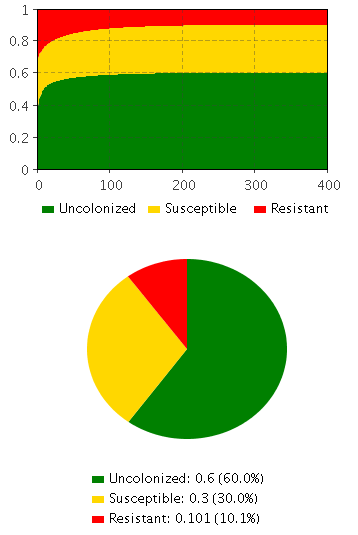
\includegraphics[height=0.7\textwidth]{img/screens/result/result1}
  \caption{The simulation dynamics of the model for the case when $R_0 > \tau_1/(\tau_1 - m \mu)$}
\end{figure}

When the basic reproductive rate is too small, the population infected by the resistant bacteria can not manage to survive under the treatment frequency of drug 2. This is why the population sharply decreases and almost disappeares from the hospital environment.

\begin{figure}[H]
  \centering
  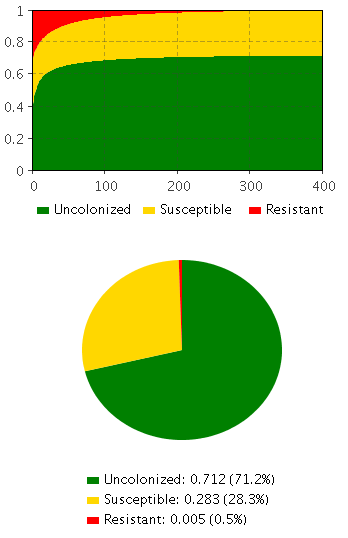
\includegraphics[height=0.7\textwidth]{img/screens/result/result2}
  \caption{Simulation results in case whent the basic reproductive rate is too small}
\end{figure}

There can be considered another extreme case, when the basic reproductive rate of the resistant strain is too high. In this case, the population infected by the resistant bacteria increases rapidly at the beginning, however becomes almost constant after some time. This phenomenon is probably happening due to presense of the second drug.

\begin{figure}[H]
  \centering
  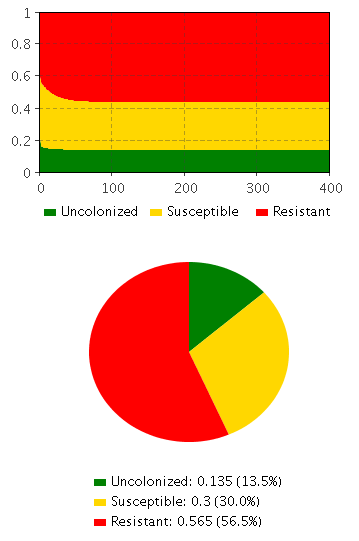
\includegraphics[height=0.7\textwidth]{img/screens/result/result3}
  \caption{Simulation with a very high basic reproductive rate}
\end{figure}
